\documentclass[11pt]{amsart}
%prepared in AMSLaTeX, under LaTeX2e
\addtolength{\oddsidemargin}{-.6in}
\addtolength{\evensidemargin}{-.6in}
\addtolength{\topmargin}{-0.6in}
\addtolength{\textwidth}{1.1in}
\addtolength{\textheight}{1.1in}
\newcommand{\normalspacing}{\renewcommand{\baselinestretch}{1.03}
        \tiny\normalsize}

\newtheorem*{thm}{Theorem}
\newtheorem*{defn}{Definition}
\newtheorem*{example}{Example}
\newtheorem*{problem}{Problem}
\newtheorem*{remark}{Remark}

\usepackage{amssymb,verbatim,fancyvrb,xspace}
\usepackage{palatino}

\usepackage[final]{graphicx}

\usepackage[pdftex, colorlinks=true, plainpages=false, linkcolor=black, citecolor=red, urlcolor=red]{hyperref}

% macros
\newcommand{\ba}{\mathbf{a}}
\newcommand{\bb}{\mathbf{b}}
\newcommand{\bn}{\mathbf{n}}
\newcommand{\br}{\mathbf{r}}
\newcommand{\bu}{\mathbf{u}}
\newcommand{\bv}{\mathbf{v}}
\newcommand{\bx}{\mathbf{x}}
\newcommand{\by}{\mathbf{y}}

\newcommand{\bT}{\mathbf{T}}

\newcommand{\CC}{\mathbb{C}}
\newcommand{\Div}{\nabla\cdot}
\newcommand{\eps}{\epsilon}
\newcommand{\grad}{\nabla}
\newcommand{\ZZ}{\mathbb{Z}}
\newcommand{\ip}[2]{\ensuremath{\left<#1,#2\right>}}
\newcommand{\lam}{\lambda}
\newcommand{\lap}{\triangle}
\newcommand{\RR}{\mathbb{R}}

\newcommand{\cond}{\operatorname{cond}}

\newcommand{\prob}[1]{\bigskip\noindent\textbf{#1}\, }
\newcommand{\ppart}[1]{\textbf{(#1)}\,\, }
\newcommand{\epart}[1]{\medskip\noindent\textbf{(#1)}\,\, }

\newcommand{\pts}[1]{\scriptsize [#1 points] \normalsize}

\newcommand{\Matlab}{\textsc{Matlab}\xspace}
\newcommand{\Octave}{\textsc{Octave}\xspace}
\newcommand{\Python}{\textsc{Python}\xspace}

\newcommand{\mfile}[2]{
	\medskip
	\begin{quote}
		\bigskip
		\VerbatimInput[frame=single,framesep=3mm,label=\fbox{\normalsize \textsl{\,#1\,}},fontfamily=courier,fontsize=\scriptsize]{#2}
		\bigskip
	\end{quote}
}

\DefineVerbatimEnvironment{mVerb}{Verbatim}{numbersep=2mm,frame=lines,framerule=0.1mm,framesep=2mm,xleftmargin=4mm,fontsize=\footnotesize}

\newcommand{\kstab}{k_{\text{stab}}}


\begin{document}
\scriptsize
\noindent Math 615 Numerical Analysis of Differential Equations \, (Bueler) \hfill  \today
\normalsize\bigskip
\normalspacing

\Large\centerline{\textbf{Solutions}}

\normalsize
\centerline{\textbf{to Worksheet:  Stable time-steps for 2nd-order ODE schemes}}

\bigskip\medskip
\thispagestyle{empty}
\normalspacing


\prob{(a)}  I computed stability functions for the first two methods:
\begin{align*}
R_{\text{TR}}(z) &= \frac{1+z/2}{1-z/2}, \\
R_{\text{EM}}(z) &= 1 + z + \frac{z^2}{2}
\end{align*}
The stability regions $S = \{z\in\CC\,:\,|R(z)|\le 1\}$ have been plotted before, and I put them together together with AB2 below.

\prob{(b)}  AB2 is a multistep method.  If we write it as
	$$U^{n+2} - U^{n+1} = z \left(\frac{3}{2} f(U^{n+1}) - \frac{1}{2} f(U^n)\right)$$
then $\rho(\zeta)=\zeta^2-\zeta$ and $\sigma(\zeta)= \frac{3}{2} \zeta - \frac{1}{2}$.  By formula (7.5),
	$$\pi(\zeta; z) = \rho(\zeta) - z\sigma(\zeta) = \zeta^2-\zeta - z\left(\frac{3}{2} \zeta - \frac{1}{2}\right) = \zeta^2-(1+\frac{3}{2}z) \zeta + \frac{1}{2}z$$
Now, the stability region $S$ is the set of $z\in\CC$ so that $\pi(\zeta; z)$ satisfies root condition (6.34), that is, so that either all roots $\zeta$ are inside the unit circle, or if there are roots on the boundary then these roots are simple.  Since $\pi(\zeta; z)$ is quadratic, we can compute its roots:
	$$\zeta = \frac{1+\frac{3}{2}z \pm \sqrt{(1+\frac{3}{2}z)^2 - 2z}}{2}$$
For a figure it suffices to check numerically that both roots have magnitudes less than 1.  Alternatively, the boundary locus method of section 7.6.1 can be used; I did both.  In fact, the following code generates the figure showing all three stability regions.

\mfile{regions.m}{regions.m}

\medskip
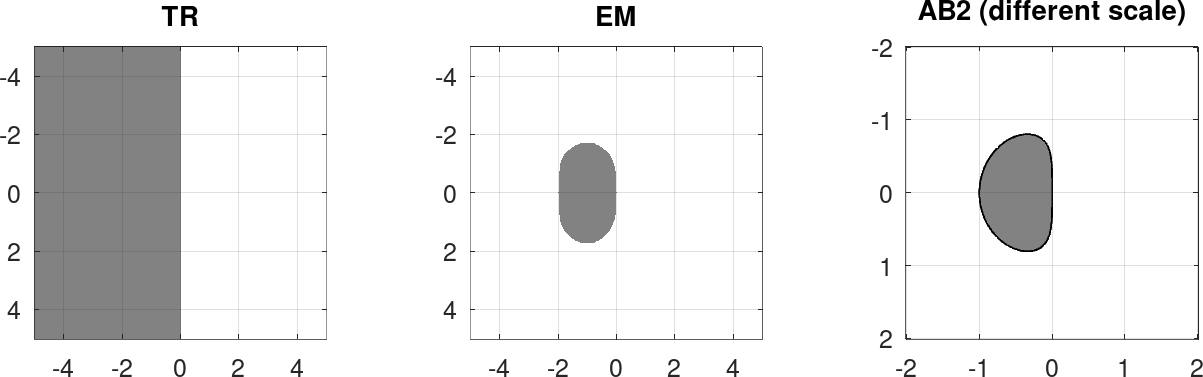
\includegraphics[width=\textwidth]{regions.png}

\medskip
\prob{(c)}  Note that the S1 and S3 matrices are symmetric, so the eigenvalues are real in those cases.  The following code finds the eigenvalues.  Note that S1 has two negative and one positive eigenvalue, both eigenvalues in S2 are purely imaginary, and S3 has only negative eigenvalues.

\mfile{alleigens.m}{alleigens.m}

Here is the result:
\begin{mVerb}
>> alleigens
S1:
  -5.56551  -0.52687  4.09237
S2:
  0 - 2i    0 + 2i
S3:
  -2694.14240  -2664.71334  -2616.14196  -2549.13655  -2464.67419  -2363.98653
  -2248.54183  -2120.02354  -1980.30573  -1831.42581  -1675.55478  -1514.96559
  -1352.00000  -1189.03441  -1028.44522   -872.57419   -723.69427   -583.97646
   -455.45817   -340.01347   -239.32581   -154.86345    -87.85804    -39.28666
     -9.85760
\end{mVerb}

\prob{(d)}  The main idea is that

\begin{quote}
\emph{For those eigenvalues $\lambda_p$ that have negative real parts, corresponding to decaying components of an exact solution, absolute stability}
    $$|U^{n+1}|\le |U^n| \,\iff\, z\in S = \{z\in\CC\,:\,|R(z)|\le 1\}$$
\emph{is a useful requirement for a reasonable time-step.  We find the largest $\kstab$ so that}
    $$z = \kstab \lambda_p$$
\emph{is in the region of absolute stability of the scheme for all $\lambda_p$ such that $\operatorname{Re}(\lambda_p)<0$.  We allow only time steps $k>0$ such that $k\le \kstab$.}
\end{quote}

For the negative eigenvalues in problem S1, absolute stability is relevant.  Since S2 has only purely-imaginary eigenvalues, absolute stability has nothing to say about it, regardless of the method.  For S3, all eigenvalues are negative so the stability restrictions for EM and AB2 are severe, with the latter worst.  For mere absolute stability,\footnote{L-stability could be considered.  Especially for S3 it suggests trying a stiff decay scheme like BDF2 instead.} trapezoid has no stability restriction on any of these methods.

Quantitatively, the $[-2,0]\subset S_{\text{EM}}$ and $[-1,0]\subset S_{\text{AB2}}$ give the largest portions of the real axis which is inside the stability region of the corresponding scheme, and this allows us to compute $\kstab$ for that scheme on systems S1 and S3.  I put my results in a table:

\bigskip
\begin{center}
\begin{tabular}{r|c|c|c}
   & \phantom{sdljf} TR \phantom{sdljf} & \phantom{sdljf} EM \phantom{sdljf} & \phantom{sdljf} AB2 \phantom{sdljf} \\ \hline
S1 & $\ast$ & $\kstab = 0.360$ & $\kstab = 0.180$\\ \hline
S2 & $\dagger$ & $\dagger$ & $\dagger$ \\ \hline
S3 & $\ast$ & $\kstab = 0.000742$ & $\kstab = 0.000371$
\end{tabular}
\end{center}

\bigskip
Certain cases need explanation:
\begin{itemize}
\item[$\ast$:]     The implicit TR method has \emph{no stability restriction} because decaying eigenvalues give decaying approximate solutions, and growing give growing.
\item[$\dagger$:]  Since all eigenvalues of S2 have zero real parts, there are \emph{no stability restrictions}.  Only $\lambda$ with $\operatorname{Re}(\lambda) < 0$ are relevant to absolute stability.
\end{itemize}

\prob{(e)}  My version of the expert advice:

\begin{itemize}
\item[S1:] I would recommend using EM subject to the given stability restriction.  One would presumably choose time steps much smaller than 0.360 anyway, for accuracy.  The reason to choose this method is ease of implementation and low computational cost, as it is an explicit method.  It is easier to implement than AB2, because EM is one-step and no start-up fiddles are required, and it is a bit more stable anyway.
\item[S2:] Any of the methods are probably o.k.~for any step size which is small enough to give decent accuracy.  But note that the eigenvalues $\lambda=\pm 2 i$ correspond to exact solution components which are purely-oscillating, with neither decay nor growth.  Because these eigenvalues correspond to points $z$ which are on the exact boundary of its stability region, method TR has the interesting property that it generates approximate solutions which also neither decay nor grow.  I would choose TR given that it is not too hard to implement on a linear problem like this.  (\emph{An observation like this explains why TR is standard for the Sch\"odinger equation: it preserves unitarity.})
\item[S3:] I would choose TR because the stability restrictions for EM and AB2 are severe, and might stop us from doing long time steps.  (\emph{That is, when a long time step would be acceptable accuracy-wise.})  Actually a scheme not tested here, namely BDF2, is a good one to recommend.  We will see that for smooth initial data both TR and BDF2 work well on discretized heat equations for essentially any time step.  But if the initial condition is rough then for large time steps TR will have worse-looking results because it does not kill off the high frequencies as it should; it is common to choose BDF2 for problems like the heat equation with rough data.
\end{itemize}

\end{document}
